\documentclass{report}
\usepackage{graphicx} % Required for inserting images
\usepackage[italian]{babel}
\usepackage{tikz}
\usepackage{hyperref}
\usepackage{amsmath}
\usepackage{xcolor}
\usepackage{float}
\usepackage{soul}
\usepackage{listings} % Per evidenziare il codice

\definecolor{lightgray}{rgb}{0.9,0.9,0.9} % Definizione colore sfondo
\definecolor{darkgreen}{rgb}{0.0, 0.5, 0.0}

\lstset{
    backgroundcolor=\color{lightgray}, % Sfondo grigio
    basicstyle=\ttfamily, % Font monospaziato
    % frame=single, % Bordo attorno al codice
    tabsize=4, % Dimensione tabulazione
    breaklines=true, % Permette di andare a capo automaticamente
    numbers = left,
    numberstyle=\small\color{gray}
}

\title{\huge\textbf{{Controllo delle Query Distribuite}}}
\date{Parte III}

\begin{document}

\maketitle
\tableofcontents
\newpage


\chapter{Introduzione}

Torniamo a preoccuparci del problema di confidenzialità, nel contesto di computazione di 
query distribuite; l'assunzione è che non tutti siano autorizzati a vedere tutti i dati, ma ci 
sono dei vincoli di confidenzialità che devono essere rispettati.

\section{Join sovrani}
Questo approccio sfrutta la presenza di un hardware fidato (nel senso che nessuno può vedere 
cosa fa), che può ricevere i dati 
per eseguire le computazioni. Lo scenario è:
\begin{itemize}
    \item si hanno due \textit{data owner} che non si fidano l'uno dell'altro
    \item c'è una terza parte, che ha a disposizione dell'hardware fidato, che esegue la computazione
\end{itemize}

\noindent L'idea è che le parti criptano i dati e li mandano all'hardware, che si occupa di:
\begin{itemize}
    \item decriptare i dati 
    \item eseguire la computazione 
    \item recriptare i dati e darli al client 
\end{itemize}

\noindent Un osservatore potrebbe inferire sulla base del risultato qualcosa, come ad esempio 
sulle dimensioni del risultato o sul tempo richiesto ad eseguire la computazione.

\noindent $\Rightarrow$ l'output deve avere più o meno sempre la stessa dimensione e tempo di computazione, 
per cercare di ridurre l'inferenza

\section{Access patterns}
Cercano di specificare come le fonti informative devono essere accedute.

\noindent Definiamo un \textit{access pattern} con un esempio:
\begin{itemize}
    \item abbiamo 3 relazioni, ciascuna con un access pattern, ovvero dei vincoli di accesso
    \item si ha una lettera per ciasuno attributo delle relazione
    \begin{itemize}
        \item $o$ per output 
        \item $i$ per input 
    \end{itemize}

    \begin{figure}[H]
        \centering
        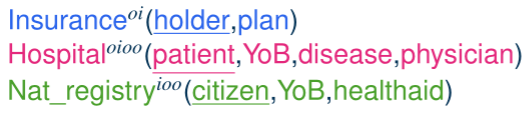
\includegraphics[width=0.6\linewidth]{images/access-pattern.png}
    \end{figure}

    \noindent \textit{per accedere all'attributo "o" mi deve dare l'attributo "i"}; si pongono dei vincoli, 
    l'accesso non è libero
\end{itemize}

\noindent Questa tecnica presenta alcuna svantaggi:
\begin{itemize}
    \item limitata espressione delle limitazioni 
    \item tipicamente ci sono due entità, non un vero scenario distribuito 
    \item può essere difficile da usare nella pratica 
\end{itemize}

\section{Autorizzazioni basate su viste}
La peculiarità di questo approccio è che le restrizioni di accesso dipendono dal contenuto del dato.

\begin{figure}[H]
    \centering
    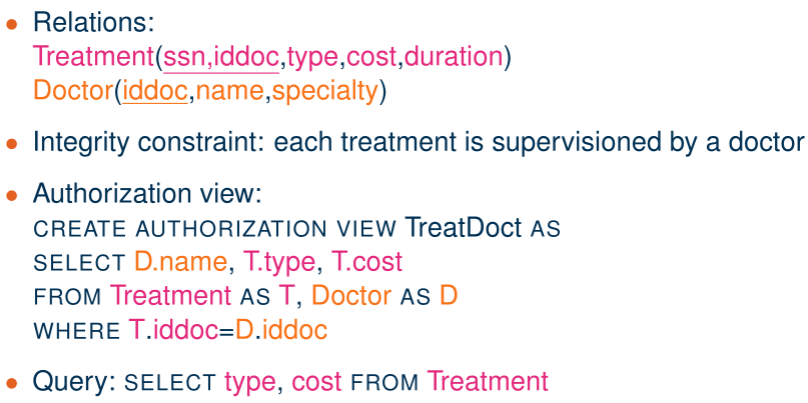
\includegraphics[width=0.8\linewidth]{images/view-auth.png}
\end{figure}

\noindent Verifico se una query può essere eseguita sulla base delle autorizzazioni che 
ho definito; il client scrive la sua query, e il server cerca di rielaborarla 
sulla base delle viste che sono state definite.

\noindent Nel caso in cui una query non possa essere eseguita, ci sono due scenari possibili:
\begin{itemize}
    \item \textit{truman:} ti restituisco un risultato parziale, che corrisponde non alla query che mi hai chiesto ma alla vista che è stata definita (facendotelo 
    passare come completo)
    \item \textit{non-truman:} non ti restituisco nulla e ti dico che non sei autorizzato ad accedere al risultato 
\end{itemize}


\section{Pairwise authorizations}
Ci sono diversi \textit{providers} che si conoscono e che formano delle \textit{coalizioni}; sono 
disposti a condividere le proprie informazioni per un obiettivo comune.

\noindent Ciascun provider ha:
\begin{itemize}
    \item una o più relazioni 
    \item uno o più server
\end{itemize}

\begin{figure}[H]
    \centering
    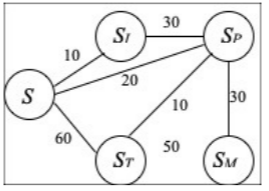
\includegraphics[width=0.4\linewidth]{images/pairwise-auth.png}
\end{figure}

\noindent I server formano una rete, possono comunicare tra di loro; una computazione vuole essere effettuata 
\textbf{minimizzando il costo} (ciascun canale a un costo asssociato) e \textbf{rispettando le restrizioni} 
sul flusso di informazioni (chi può vedere che cosa).


\noindent $\Rightarrow$ Si definisce un \textit{\textbf{safe query plan}}, ovvero un modo per soddsifare la query in modo 
sicuro e che minimizzi i costi:
\begin{itemize}
    \item per le operazioni unarie non ci sono problemi, dato che non richiedono alcun trasferminento di dati 
    \item per le operazioni di join, viene richiesto la cooperazione tra i due server:
    \begin{itemize}
        \item uno funge da \textit{master}, ha il compito di eseguire il join 
        \item uno funge da \textit{slave}, aiuta il master
    \end{itemize}
\end{itemize}

\subsection{Broker join}
Ci sono due relazioni su due server, su cui dobbiamo eseguire il join. Tipicamente, uno 
dei due server funge da master e l'altro da slave; se però sono state definite delle restrizioni 
che impediscono di accedere all'altra relazione, questa architettura non può esssere utilizzata.

\noindent Con il broker-join si usa (se esiste) un terzo server che sia autorizzata ad accedere alle relazioni 
ed eseguire il join; se ne esistono più di uno, seleziono quello con il costo minore.

\subsection{Peer-join}
Sfrutto entrambi i server, perché entrambi sono autorizzati ad accedere all'altra relazione; il join 
viene eseguito in modo che uno dei due server manda la tabella all'altro, che eseguirà il join 
per poi dare il risultato al client.





\end{document}
